\documentclass{article}

\usepackage{extramarks}

\usepackage{amsmath}
\usepackage{amsthm}
\usepackage{amssymb}
\usepackage{amsfonts}
\usepackage{caption}
\usepackage{subcaption}
\usepackage{listings}

\usepackage{hyperref}

\usepackage{tikz}

\usepackage{algorithm}
\usepackage{algorithmic}
\usepackage[shortlabels]{enumitem}

\usepackage{float,graphicx}

\usepackage{pgfplots}

\usepackage{adjustbox}


\usepackage{array}
\usepackage{pgfgantt}

\usepackage[utf8]{inputenc}

\usepackage{fancyhdr}
\usepackage{fancybox}

\topmargin=-0.45in
\evensidemargin=0in
\oddsidemargin=0in
\textwidth=6.5in
\textheight=9.0in
\headsep=0.25in

% Listings' Styles

\definecolor{codegreen}{rgb}{0,0.6,0}
\definecolor{codegray}{rgb}{0.5,0.5,0.5}
\definecolor{codepurple}{rgb}{0.58,0,0.82}
\definecolor{backcolour}{rgb}{0.96,0.96,0.96}


\lstdefinestyle{python}{
    backgroundcolor=\color{backcolour},
    commentstyle=\color{codegreen},
    keywordstyle=\color{magenta},
    numberstyle=\tiny\color{codegray},
    stringstyle=\color{codepurple},
    basicstyle=\footnotesize,
    breakatwhitespace=false,
    breaklines=true,
    captionpos=b,
    keepspaces=true,
    numbers=left,
    numbersep=5pt,
    showspaces=false,
    showstringspaces=false,
    showtabs=false,
    tabsize=2
}

\lstset{style=python}
\lstset{language=Python}

\linespread{1.1}
\captionsetup[table]{position=bottom}

\pagestyle{fancy}
\lhead{\groupName}
\chead{\hmwkClass: \hmwkTitle}
\rhead{\today}
\lfoot{\lastxmark}
\cfoot{\thepage}

\renewcommand\headrulewidth{0.4pt}
\renewcommand\footrulewidth{0.4pt}
\renewcommand\qedsymbol{$\blacksquare$}

\setlength\parindent{0pt}

\newcommand{\hmwkTitle}{Assignment Sheet\ \#\hmwkNumber}
\newcommand{\hmwkDueDate}{March 8, 2022}
\newcommand{\hmwkClass}{Machine Learning}
\newcommand{\hmwkAuthorName}{Henri Sota, Enis Mustafaj}
\newcommand{\groupName}{\textbf{Group HB}}

% Homework Number Variable
\newcommand{\hmwkNumber}{4}

%
% Create Problem Sections
%

\newcommand{\enterProblemHeader}[1]{
    \nobreak{}
}

\newcommand{\exitProblemHeader}[1]{
    \stepcounter{#1}
}

\setcounter{secnumdepth}{0}
\newcounter{partCounter}
\newcounter{homeworkProblemCounter}

\setcounter{homeworkProblemCounter}{1}
\nobreak\extramarks{Problem \hmwkNumber \arabic{homeworkProblemCounter}}{}\nobreak{}

%
% Homework Problem Environment
%
% This environment takes an optional argument. When given, it will adjust the
% problem counter. This is useful for when the problems given for your
% assignment aren't sequential. See the last 3 problems of this template for an
% example.
%
\newenvironment{homeworkProblem}[1][-1]{
    \ifnum#1>0
        \setcounter{homeworkProblemCounter}{\hmwkNumber.#1}
    \fi
    \section{Problem \hmwkNumber.\arabic{homeworkProblemCounter}}
    \setcounter{partCounter}{1}
    \enterProblemHeader{homeworkProblemCounter}
}{
    \exitProblemHeader{homeworkProblemCounter}
}


\newcounter{programmingPartCounter}
\newcounter{programmingProblemCounter}

\setcounter{programmingProblemCounter}{1}
\nobreak\extramarks{Programming Problem \hmwkNumber \arabic{programmingProblemCounter}}{}\nobreak{}

%
% Programming Problem Environment
%
% This environment takes an optional argument. When given, it will adjust the
% problem counter. This is useful for when the problems given for your
% assignment aren't sequential. See the last 3 problems of this template for an
% example.
%
\newenvironment{programmingProblem}[1][-1]{
    \ifnum#1>0
        \setcounter{programmingProblemCounter}{\hmwkNumber.#1}
    \fi
    \section{Programming Problem \hmwkNumber.\arabic{programmingProblemCounter}}
    \setcounter{programmingPartCounter}{1}
    \enterProblemHeader{programmingProblemCounter}
}{
    \exitProblemHeader{programmingProblemCounter}
}

\title{
    \vspace{2in}
    \textmd{\textbf{\hmwkClass:\\ \hmwkTitle}}\\
    \normalsize\vspace{0.1in}\small{Due\ on\ \hmwkDueDate\ at 10:00}\\
    \vspace{3in}
}

\author{\groupName \\ \hmwkAuthorName}
\date{}

\renewcommand{\part}[1]{\textbf{\large Part \Alph{partCounter}}\stepcounter{partCounter}\\}

% Useful for algorithms
\newcommand{\alg}[1]{\textsc{\bfseries \footnotesize #1}}

% Alias for the Solution section header
\newcommand{\solution}{\textbf{\large Solution}}
\newcommand{\comment}[1]{} % Multi-line comment


\begin{document}
\maketitle
\pagebreak
\begin{homeworkProblem}
In this task, we revise Examples 3.2 and 3.3 from the lecture notes for a different setup:

Let $X : \Omega \to \mathbb{R}$ be an input variable and $Y : \Omega \to \mathbb{R}$ be an output variable. For the input variable we assume that it follows the uniform distribution as $X \sim \mathcal{U}[-1, 1]$. (Note the other range!) Moreover, we make the very strong assumption to know the "true" dependency between $X$ and $Y$. Specifically we define $Y$ via
\begin{equation*}
    Y := g(X), \quad \text{with} \quad g(x) = x^{4}
\end{equation*}

Now we look for a function $f$ that shall approximate that (usually unknown) relationship between $X$ and $Y$. We claim that
\begin{equation*}
    f(x) = x^{3}
\end{equation*}
is a good approximation to $Y = g(X)$.

\begin{enumerate}[a)]
    \item Calculate the expected (squared) prediction error for $f$. Why is the error that large compared to the lecture example?
    \begin{equation*}
        EPE(f) = E[L_{2}(y, f(x)] = \int_{R} \int_{R} ((y - f(x))^{2} p(x, y) \: dx dy
    \end{equation*}

    Based on Knowledge 3.1, it is possible to substitute the joint density with the product of the marginal density of $X$ and a Dirac Delta function, and then use the Dirac Delta function to integrate with regards to $y$.
    \begin{equation*}
        \begin{split}
            EPE(f) & = \int_{R} \int_{R} (y - x^{3})^{2} p_{X}(x) \delta(y - x^{4}) \: dx dy \\
            & = \int_{R} \int_{R} (y - x^{3})^{2} p_{X}(x) \delta(y - x^{4}) \: dy dx \\
            & = \int_{R} p_{X}(x) \int_{R} (y - x^{3})^{2} \delta(y - x^{4}) \: dy dx \\
            & = \int_{R} p_{X}(x) (x^{4} - x^{3})^{2} \: dx \\
        \end{split}
    \end{equation*}

    Since we know that $X$ is uniformly distributed in the range $[-1, 1]$, the marginal density will be equal to 0.5 in that interval and 0 everywhere else.
    \begin{equation*}
        \begin{split}
            EPE(f) & = \frac{1}{2} \int_{-1}^{1} (x^{4} - x^{3})^{2} \: dx \\
            & = \frac{1}{2} \int_{-1}^{1} (x^{8} - 2 x^{7} + x^{6}) \: dx \\
            & = \frac{1}{2} \left[ \frac{x^{9}}{9} - \frac{x^{8}}{4} + \frac{x^{7}}{7} \right]_{-1}^{1} \\
            & = \frac{1}{2} \left[ \left (\frac{1}{9} - \frac{1}{4} + \frac{1}{7}\right) - \left(-\frac{1}{9} - \frac{1}{4} - \frac{1}{7}\right) \right] \\
            & = \frac{1}{2} \left(\frac{2}{9} + \frac{2}{7}\right) \\
            & = \frac{16}{63} \\
            & \approx 0.254
        \end{split}
    \end{equation*}

    The error is large compared to the lecture example due to the extended range $[-1, 1]$ and due to the difference between an odd ($x^{3}$) and even function ($x^{4}$) on the negative domain.

    \item Find the regressor for $Y = g(X)$.

    Using Knowledge 3.1, we can retrieve the dependency of $Y$ on $X$ by using the conditional density of $Y$ given $X$.
    \begin{equation*}
        p(y | x) = \frac{p(x, y)}{p_{X}(x)} = \frac{\delta(y - x^{4}) p_{X}(x)}{p_{X}(x)} = \delta(y - x^{4})
    \end{equation*}

    Evaluating the regressor using the Dirac Delta function to integrate with regards to $y$:
    \begin{equation*}
        \begin{split}
            E[Y | X] & = \int_{R} y p(y | x) \: dy \\
            & = \int_{R} y  \delta(y - x^{4}) \: dy \\
            & = y \\
            & = x^4
        \end{split}
    \end{equation*}
\end{enumerate}
\end{homeworkProblem}

\begin{homeworkProblem}
In the lecture slides, you have seen that the expected (squared) prediction error $EPE(f)$ is given by
\begin{equation*}
    EPE(f) = E(L_{2}(Y, f(X))
\end{equation*}

Theorem 3.1 then states that the function $f$ that minimizes the expected (squared) prediction error $EPE(f)$ is given by
\begin{equation*}
    f(x) = E(Y | X = x)
\end{equation*}

Note that in the middle of the proof, we encounter an equation
\begin{equation*}
    \begin{split}
        EPE(f) & = E_{X} E_{Y | X} [ (f(X) - E[Y | X])^{2} + 2(f(X) - E[Y | X])(E[Y | X] - Y) + (E[Y | X] - Y)^{2}| X]
    \end{split}
\end{equation*}
where the second term can be dropped. Now, prove that this is possible, i.e. that it holds
\begin{equation*}
    2 E_{X} E_{Y | X} [(f(X) - E[Y | X])(E[Y | X] - Y) | X] = 0
\end{equation*}

From the above statement we can derive that:
\begin{equation*}
    E_{X} E_{Y | X} [(f(X) - E[Y | X])(E[Y | X] - Y) | X] = 0
\end{equation*}
By expanding the statement inside the first expected value we get:
\begin{equation*}
    E_{X} E_{Y | X} [E[Y|X] \cdot f(x) - Y \cdot f(x) - E[Y|X]^{2} + Y \cdot E[Y|X]| X] = 0
\end{equation*}
In order for the equation to be 0, the term:
\begin{equation*}
    E_{Y | X} [E[Y|X] \cdot f(x) - Y \cdot f(x) - E[Y|X]^{2} + Y \cdot E[Y|X]| X]
\end{equation*}
needs to be $0$.
Now we expand the expected value with regard to the terms inside:
\begin{equation*}
    E[E[Y|X] \cdot f(x) | X] - E[Y \cdot f(x) | X] - E[E[Y|X]^{2} | X] + E[Y \cdot E[Y|X]| X] = 0
\end{equation*}
By using the property of the expected value that if 2 events $A$ and $B$ are independent of each other, then:
\begin{equation*}
    E[A \cdot B] = E[A] \cdot E[B]
\end{equation*}
we get:
\begin{equation*}
    E[E[Y|X] | X] \cdot E[f(x) | X] - E[Y | X] \cdot E[f(x) | X] - E[E[Y|X] | X] \cdot E[E[Y|X] | X] + E[Y | X] \cdot E[E[Y|X] | X] = 0
\end{equation*}
By simplifying:
\begin{equation*}
    E[E[Y|X]|X] = E[Y|X]
\end{equation*}
we get:
\begin{equation*}
    E[Y|X] \cdot E[f(x) | X] - E[Y | X] \cdot E[f(x) | X] - E[Y|X] \cdot E[Y|X] + E[Y | X] \cdot E[Y|X] = 0
\end{equation*}

From the equation we can see that the terms cancel each other and the result will be $0$.

\end{homeworkProblem}
\begin{homeworkProblem}
You are given the following training data:
\begin{equation*}
\resizebox{1.0 \textwidth}{!}{
    $ \mathcal{T} = \left\{ \left( (1,7)^{\top}, 15 \right), \left( (2,5)^{\top}, 21 \right), \left( (2,6)^{\top}, 32 \right), \left( (3,3)^{\top}, 32 \right), \left( (3,2)^{\top}, 25 \right), \left( (3,1)^{\top}, 1 \right), \left( (4,2)^{\top}, 14 \right), \left( (5,4)^{\top}, 18 \right), \left( (5,6)^{\top}, 12 \right) \right\} $
}
\end{equation*}

Manually carry a kNN regression prediction for $\mathbf{x}_{1} = (3, 3)^{\top}$, $\mathbf{x}_{2} = (3, 6)^{\top}$, $\mathbf{x}_{3} = (5, 3)^{\top}$, and $k = 1, k = 3, k = 6$. As part of the task, you have to draw the points in a scatter plot (on paper) and mark the respective neighborhoods that contribute to the final result.

\begin{figure}[h!]
    \centering
    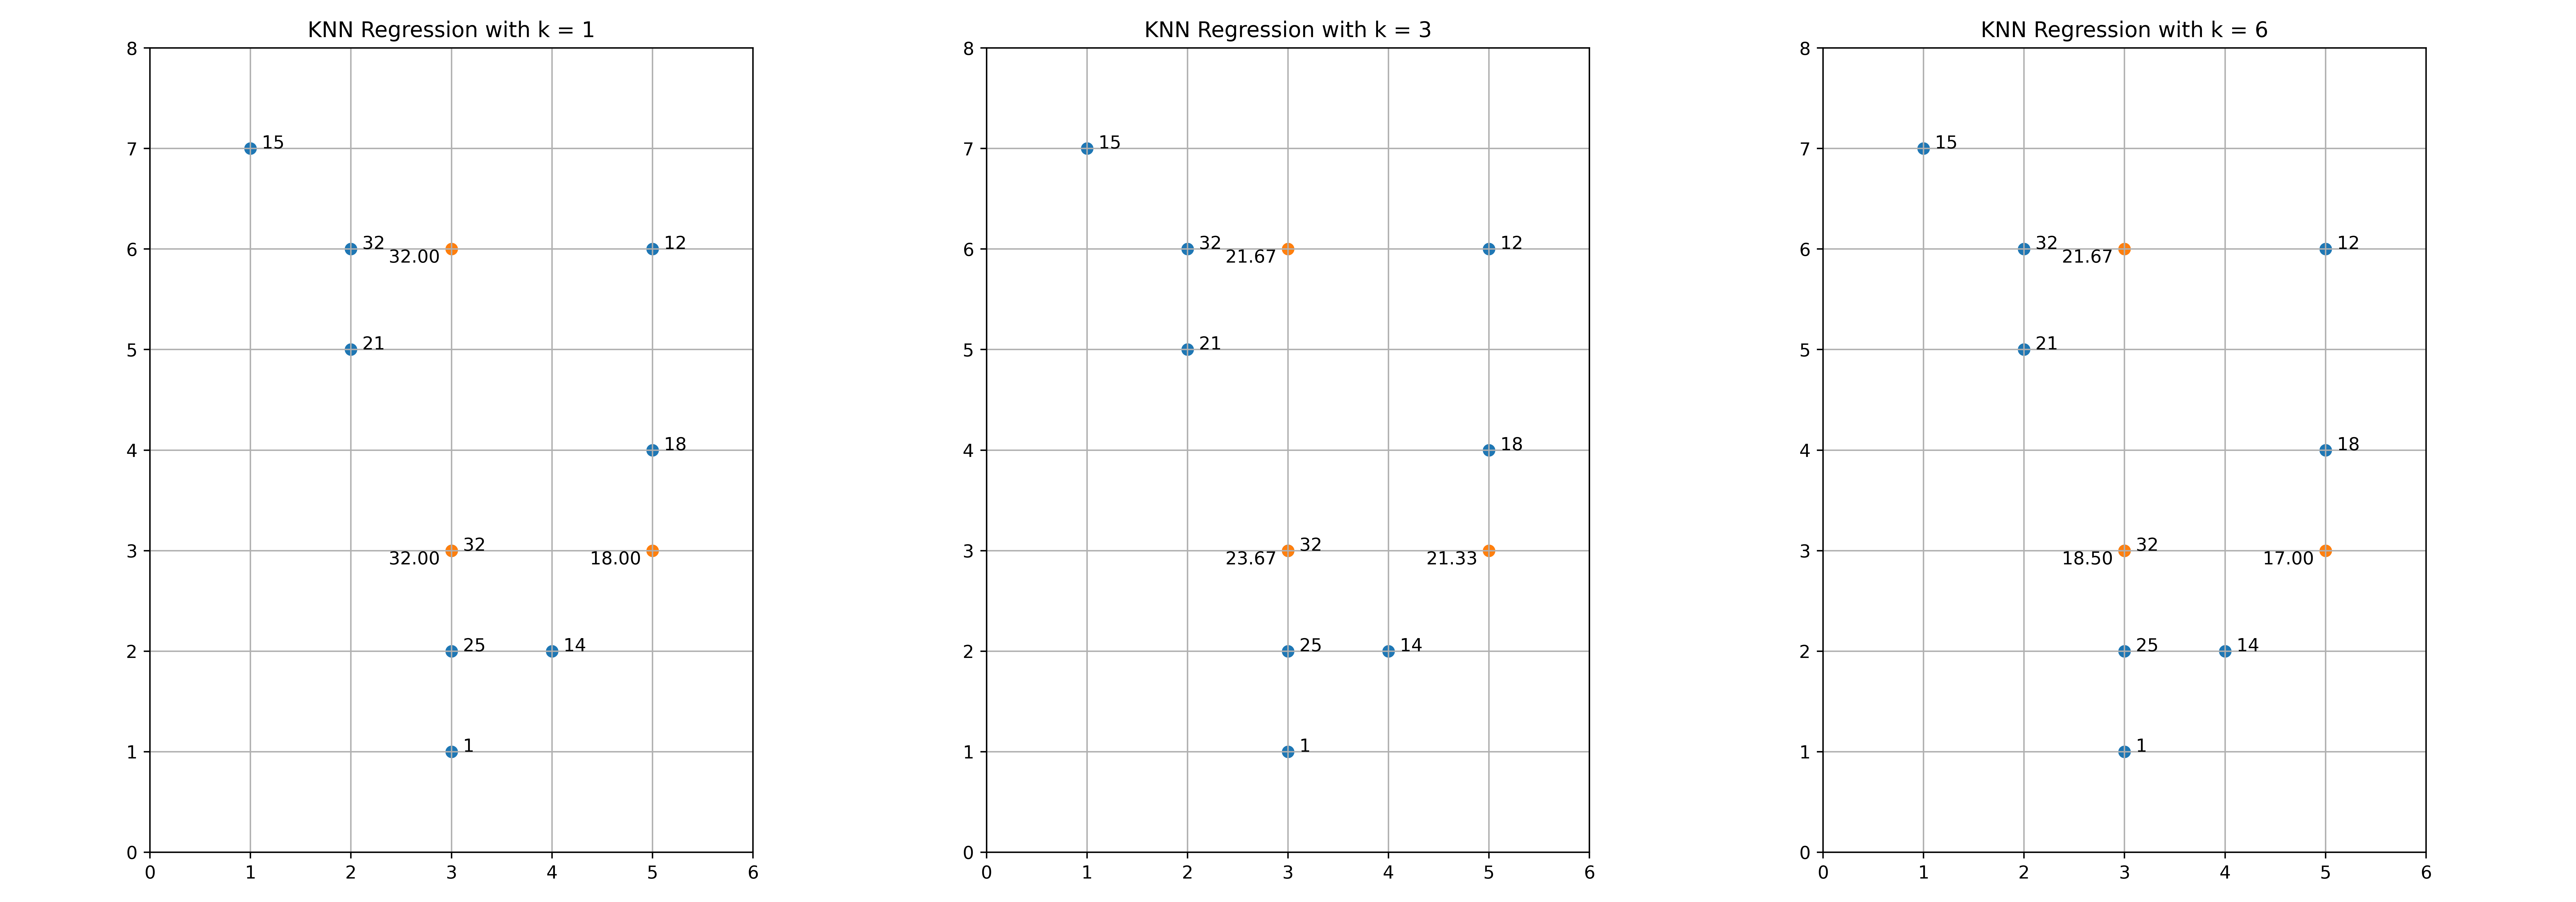
\includegraphics[width=\textwidth]{images.png}
\end{figure}

\begin{itemize}
    \item k = 1
        \begin{itemize}
            \item The nearest neighbour of the point $x_{1} = (3, 3)^{T}$ is the point $(3, 3)^{T}$ itself so the result of KNN regression will be $32$
            \item The nearest neighbour of the point $x_{2} = (3, 6)^{T}$ is the point $(2, 6)^{T}$. The result of KNN regression will be $32$
            \item The nearest neighbour of the point $x_{3} = (5, 3)^{T}$ is the point $(5, 4)^{T}$. The result of KNN regression will be $18$
        \end{itemize}
    \item k = 3
        \begin{itemize}
            \item The 3 nearest neighbours of the point $x_{1} = (3, 3)^{T}$ are the points $(3, 3)^{T}, (3, 2)^{T}, (4, 2)^{T}$. The the result of KNN regression will be $\frac{32 + 25 + 14}{3} = 23.67$
            \item The 3 nearest neighbours of the point $x_{2} = (3, 6)^{T}$ are the points $(2, 5)^{T}, (2, 6)^{T}, (5, 6)^{T}$. The the result of KNN regression will be $\frac{32 + 21 + 12}{3} = 21.67$
            \item The 3 nearest neighbours of the point $x_{3} = (5, 3)^{T}$ are the points $(5, 6)^{T}, (4, 2)^{T}, (3, 3)^{T}$. The the result of KNN regression will be $\frac{32 + 18 + 14}{3} = 21.33$
        \end{itemize}
    \item k = 6
        \begin{itemize}
            \item The 6 nearest neighbour of the point $x_{1} = (3, 3)^{T}$ are the points $(3, 3)^{T}, (3, 2)^{T}, (4, 2)^{T}, (3, 1)^{T}, \\ (5, 4)^{T}, (2, 5)^{T}$ itself so the result of KNN regression will be $\frac{32 + 25 + 1 + 18 + 14 + 21}{6} = 18.5$
            \item The 6 nearest neighbour of the point $x_{2} = (3, 6)^{T}$ are the points $(3, 3)^{T}, (2, 6)^{T}, (2, 5)^{T}, (5, 6)^{T}, \\ (1, 7)^{T}, (5, 4)^{T}$ itself so the result of KNN regression will be $\frac{32 + 18 + 12 + 32 + 21 + 15}{6} = 21.67$
            \item The 6 nearest neighbour of the point $x_{1} = (5, 3)^{T}$ are the points $(3, 3)^{T}, (3, 2)^{T}, (3, 1)^{T}, (4, 2)^{T}, \\ (5, 4)^{T}, (5, 6)^{T}$ itself so the result of KNN regression will be $\frac{32 + 25 + 1 + 14 + 18 + 12}{6} = 17$
        \end{itemize}
\end{itemize}


\end{homeworkProblem}

\begin{programmingProblem}
Consider the Examples 3.4 and 3.5 from the lecture, for which you also have access to the source code. Complete the following tasks:

\begin{enumerate}[a)]
    \item (Re-)implement Example 3.4. This time, however, you need to implement the kNN regression by yourself, without a machine learning library and without a kNN search library. (If you implement in Python, just start from the available Jupyter notebook) Verify the correctness of your implementation by cross-checking it with Example 3.4.
    \item Apply your implementation to the Energy efficiency Data Set from the UCI Machine Learning Repository. Build the predictor for the required heating load on the full data set and predict the load on the first three samples of the data set and $k = 1$, $k = 3$, $k = 10$.
    \item (Re-)implement Example 3.5. This time, however you need to implement the kNN classification by yourself, without a machine learning library and without a kNN search library. (If you implement in Python, just start from the available Jupyter notebook) Verify the correctness of your implementation by cross-checking it with Example 3.5.
    \item Now, we would like to use kNN classification for SPAM classification. Either you collect some e-mails (both SPAM and no SPAM) from your Inbox, label them manually and create the representation using your implementation from last week or you use the Spambase Data Set from the UCI Machine Learning Repository. Apply your implementation to one of these data sets and evaluate the predictor for three random samples in the data set and values $k = 1$, $k = 3$, $k = 10$. Compare these results to the training data.
\end{enumerate}

The implementation of the kNN regressor and classifier can be found in the file \texttt{programming\_exercises.ipynb}. Both have been implemented as classes that can be instantiated given the \texttt{n\_neighbors} argument which is the number of neighbors used when searching for the neighbors of data point. The classes offer two methods, \texttt{fit} and \texttt{predict}, which add the data to the model and predict the expected regression value or class respectively.
\end{programmingProblem}

\end{document}
